\let\negmedspace\undefined
\let\negthickspace\undefined
\documentclass[journal]{IEEEtran}
\usepackage[a5paper, margin=10mm, onecolumn]{geometry}
%\usepackage{lmodern} % Ensure lmodern is loaded for pdflatex
\usepackage{tfrupee} % Include tfrupee package

\setlength{\headheight}{1cm} % Set the height of the header box
\setlength{\headsep}{0mm}     % Set the distance between the header box and the top of the text
\usepackage{gvv-book}
\usepackage{gvv}
\usepackage{cite}
\usepackage{amsmath,amssymb,amsfonts,amsthm}
\usepackage{algorithmic}
\usepackage{graphicx}
\usepackage{textcomp}
\usepackage{xcolor}
\usepackage{txfonts}
\usepackage{listings}
\usepackage{enumitem}
\usepackage{mathtools}
\usepackage{gensymb}
\usepackage{comment}
\usepackage[breaklinks=true]{hyperref}
\usepackage{tkz-euclide} 
\usepackage{listings}
% \usepackage{gvv}                                        
\def\inputGnumericTable{}                                 
\usepackage[latin1]{inputenc}                                
\usepackage{color}                                            
\usepackage{array}                                            
\usepackage{longtable}                                       
\usepackage{calc}                                             
\usepackage{multirow}                                         
\usepackage{hhline}                                           
\usepackage{ifthen}                                           
\usepackage{lscape}
\begin{document}

\bibliographystyle{IEEEtran}
\vspace{3cm}

\title{1.1.8.26}
\author{EE24BTECH11047 - Niketh Prakash Achanta}
% \maketitle
% \newpage
% \bigskip
{\let\newpage\relax\maketitle}

\renewcommand{\thefigure}{\theenumi}
\renewcommand{\thetable}{\theenumi}
\setlength{\intextsep}{10pt} % Space between text and floats
\numberwithin{equation}{enumi}
\numberwithin{figure}{enumi}


\renewcommand{\thetable}{\theenumi}


\textbf{Question}:\\
Find a point on the Y axis which is equidistant from the points $\vec{A}\myvec{6,5}$ $\vec{B}\myvec{-4,3}$.\\
\\ \solution \\
    \begin{table}[h!]    
      \centering
      \begin{tabular}[12pt]{ |c| c|}
    \hline
    \textbf{Variable} & \textbf{Description}\\ 
    \hline
    $A$ & One end of line segment \\
    \hline 
    $B$ & Other end of line segment \\
    \hline
    $P_1$ & First point of trisection \\
    \hline
    $P_2$ & Second point of trisection \\
    \hline
    $m$ & Ratio in which $P_1$ divides AB \\
    \hline
    $n$ & Ratio in which $P_2$ divides AB \\
    \hline
    \end{tabular}

      \caption{}
    \end{table}\\
If $\vec{P}$ is equidistant from the points $\vec{A}$ and $\vec{B}$
    \begin{align}
        \abs{\abs{\vec{P}-\vec{A}}} = \abs{\abs{\vec{P}-\vec{B}}} \label{eq1.1.9.17.1}
    \end{align}
     \begin{align}
        \abs{\abs{\vec{P}-\vec{A}}}^2 = \abs{\abs{\vec{P}-\vec{B}}}^2\label{eq1.1.9.17.2}
    \end{align}
    \begin{align}
    	\abs{\abs{\vec{P}}}^2 - 2\vec{P}^\top \vec{A} + \abs{\abs{\vec{A}}}^2 = \abs{\abs{\vec{P}}}^2 - 2\vec{P}^\top\vec{B} + \abs{\abs{\vec{B}}}^2\label{eq1.1.9.17.3}
    \end{align}
By simplifying further,
    \begin{align}
    	\brak{\vec{A}-\vec{B}}^\top \vec{P} = \frac{\abs{\abs{\vec{A}}}^2-\abs{\abs{\vec{B}}}^2}{2} \\
    	\myvec{10 \\ 2}^\top \vec{P} = \frac{\abs{\abs{\myvec{6 \\ 5}}}^2-\abs{\abs{\myvec{-4 \\ 3}}}^2}{2} = 18\label{eq1.1.9.17.4}
    \end{align}
Comparing with $n^\top x = c$
    \begin{align}
    	\vec{n} = \myvec{10 \\ 2}\\ \label{eq1.1.8.28.5}
	    \vec{c} = 18\\
     10x+2y=18\\
     x=0,y=9\\
     \vec{P}=\myvec{0 \\ 9}
    \end{align}
    \begin{figure}[h]
        \centering
       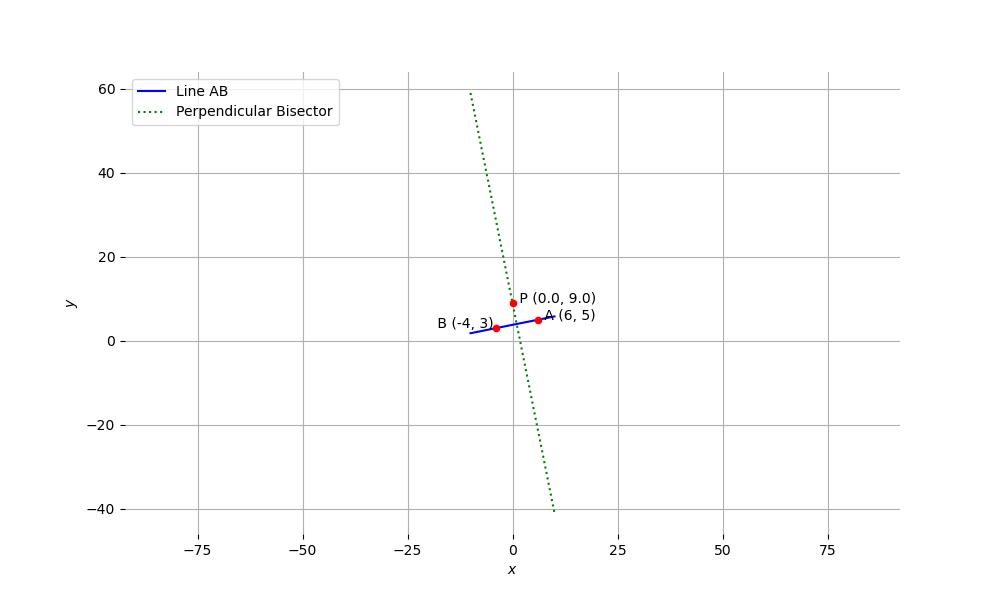
\includegraphics[width=\linewidth]{figs/fig1.png}
       \caption{}
       \label{graph}
    \end{figure}



\end{document}  







